% !TEX root = ../Survey.tex
	In this section we describe results relevant to the \adjacency function.
	We begin the section by a literature overview. 
	Section~\ref{sec-adj-lb} is dedicated to the current best bound.
	We begin it by showing two  $\log n + O( \log \log n)$ \adjacency labeling schemes.
	Those are a stepping stone to an improved $\log n+O(\log^* n)$ labeling scheme, which is described in detail.
	 Section~\ref{traversaljumping} surveys the technique, ``traversal and jumping'', for \adjacency in  caterpillars.
	 In addition, we sketch a new optimal labeling scheme for bounded degree trees.
	 Finally, in Section~\ref{sec-adj-onesided} we discuss the one-sided error variant.
\subsection{Literature overview}
	\adjacency labeling schemes were introduced by \citeN{Breuer67}, and revisited by \citeN{Kannan92} for trees and graphs.
	They were also independently defined by \citeN{Muller1988} in a model that does not require polynomiality of encoding and decoding.
	Following the $2 \log n$ \adjacency labeling schemes for trees (Section~\ref{sec:example}), Abiteboul, Kaplan, and Milo \shortcite{Kaplan01} improved the label size to $1.5 \log n+O(\log \log n)$.
	\citeN{Alstrup02} proved that both $Forests(n)$ and $Trees(n)$ have an \adjacency  labeling scheme of $\log n +O(\log^*n)$.
	Recently, ~\citeN{Fraigniaud10} showed  that trees with bounded depth $\delta$ have a labeling scheme of size $\log n+ 3\log \delta +O(1)$.
\citeN{Gavoille06}  proved that caterpillars and binary trees enjoy a labeling scheme of size $\log(n)+O(1)$ using a method called ``Traversal and jumping''.
	~\citeN{adjiashvili2014labeling} showed that trees with bounded degree $\Delta$ have a labeling scheme of size $\log n + \log \Delta + O(1)$.  
		~\citeN{fraigniaud2009}  showed that in a one-sided error labeling scheme, \nonadjacency labeling schemes require $k+1$ bits to have a guarantee of $1-\frac{1}{2^k}$.
		
	\adjacency labeling schemes for trees are useful for general graphs due to an observation  by 	
	\citeN{nash1961edge}, which states that a graph of arboricity\footnote{The arboricity of a graph $G$  is the minimum number of edge-disjoint acyclic subgraphs whose union is $G$.
}  $d$  can be decomposed into  at most $d$ forests\footnote{See also~\cite{chen1994short} for a simplified proof of the claim.}. \citeN{Kannan92} proved that graphs with arboricity $d$ can be labeled using $(d+1) \log n$ bit labels.
	Therefore, the labeling scheme of \citeN{Alstrup02}  yields a label size of $d\log n +O(log^* n)$ for graphs with arboricity $d$.Graphs in $\mathcal{G}(n,\Delta)$ have arboricity of $\ceil{ \Delta  / 2} $~\cite{Kannan92}.
	It follows that graphs in $\mathcal{G}(n,\Delta)$  have a labeling scheme of  $(\lceil \Delta  / 2 \rceil) \log n  +O(log^* n) $ bits if $\Delta$ is constant.


%\paragraph{Using labeling scheme to construct an induced-universal graph}	
\subsection{Upper bound for $Trees(n)$ }\label{sec-adj-lb}
For general trees,  \citeN{Alstrup02} showed a $\log n+{O}(\log^* n)$ labeling scheme for \adjacency with query time of $O(\log^* n)$ and encoding time of $O(n \log^*n)$.
In this section we describe their result in detail.

\subsubsection{An \adjacency labeling scheme of $\log n +O(\log \log n$) bits}\label{sec-adj-simple}
We first introduce two labeling schemes for $Trees(n)$.
The first favours equal size labeling scheme for all nodes, and the other   achieves a smaller label size for leaves, at the expanse of bigger label size for internal nodes.
\begin{lemma} \cite{Alstrup02}\label{lem:4loglogn}\label{Lemma-adj-loglogn}
The following  \adjacency labeling schemes are available for  $Trees(n)$.
$ \tuple{e_\alpha,d_\alpha}$, whose worst-case label size is  $\log n + 3\log \log n $ for all nodes, and $ \tuple{e_\beta,d_\beta}$, which has a label size of  $\log n +O(1)$ for the leaves and $\log n + 4\log \log n$ for internal  nodes.
\end{lemma}
 
Both labeling schemes are based on a heavy-light decomposition (Section~\ref{tec:heavylight}) as well as a $\dfsi$ traversal (Section~\ref{tec:dfs}), in which children of small size are visited before children of larger size.
They also use $1/2$-approximation (see Section~\ref{section:Misc-Tools}) of  numbers in $\{1 \dots n\}$ for different parts of the labels.

Consider a non-leaf  node $v$ with parent $p(v)$ and heavy child $h$.
The encoder of $\tuple{e_\alpha,d_\alpha}$ labels $v$ as a concatenation of  the bit strings:
\begin{inparaenum}[\itshape I.\upshape)]
  \item~$\dfsi(v)$;
 \item~$\ldepth(v)$;
 \item~a $1/2$-approximation of $\dfsi(v)-\dfsi(p(v))$; and
 % denoted $\lfloor o \rfloor_2(v)$
\item~a $1/2$-approximation of $\dfsi(h)-\dfsi(v)$.
  %denoted $\lfloor ls \rfloor_2(v)$.
 \end{inparaenum}
Leaves are labeled similarly, with  the last part set to $0$, and the root is marked especially.

%Suppose  $u$ is  the  parent of the  light node   $v$.
%The decoder  $d_\alpha$ returns true for  $\la(u),\la(v)$ by verifying  the following predicates hold:
%\begin{itemize}
%\item $\dfsi(u)< \dfsi(v)$.
%\item $\ldepth(v) = \ldepth(u)+1$.
%\item  $ \lfloor ls \rfloor_2(u) \geq \lfloor o \rfloor_2(v)$. 
%\item  compute a $1/2$ approximation  of $pre(u)-pre(v)$ and return true if it is equal to  $\lfloor o \rfloor _2(v)$.
%\end{itemize}
%If $v$ is a heavy node, the query  is verified similarly  with the exceptions that now the light depths are equal, and that $\lfloor ls \rfloor_2(u) = \lfloor o \rfloor _2(v)$. 
%
%Assume in contradiction that the conditions hold, and $u$ is not the parent of $v$.
%The two first predicates assure that $u$ can not be a descendant of $v$. So the path $u \leadsto v$ in $T$ must contain $p(p(v)$. The nodes between $u$ and its heavy node $h_u$ and  those between $p(v)$ and $v$ must have been traversed before $v$ in the $\dfsi$ traversal, which implies that $\dfsi(v)-\dfsi(u) \geq  \dfsi(v)-\dfsi(p(v)) + \dfsi(h_u)-\dfsi(u)$.
%On the other hand, we know that $ \lfloor ls \rfloor_2(u) \geq \lfloor o \rfloor_2(v)$

\citeN{Alstrup02} prove that the information is sufficient to determine adjacency.
For convenience, it is provided in App.~\ref{AppendixB}.
 %The proof that the information described is  sufficient to determine adjacency is found in~\cite{Alstrup05} (Section~3.1).

We create $\tuple{e_\beta,d_\beta}$ by  extending $\tuple{e_\alpha,d_\alpha}$ such that  each internal node  receives  additional $\log \log n$ bits, describing a   $1/2$-approximation  of  the number of  its leaf children, which we denote $\lfloor{l}\rfloor_2$.
Suppose  that $v$ and $u$ are two leaf children of a node with $l$ children, and $v$ is one of the first  $\lfloor{l}\rfloor_2$ leaf children  traversed, and $u$ is not.
The encoder then sets  $\la(v) = (\dfsi(v),0)$  and $\la(u) = (\dfsi(u)-\lfloor{l}\rfloor_2,1)$.
See Figure~\ref{fig:bitTricks} for  a demonstration.
In conclusion, $\tuple{e_\beta,d_\beta}$ produces labels of size $\log n + 4 \log \log n$  for internal nodes and $\log n +O(1)$ for leaves.

 
 				\begin{figure} 
				\centering
				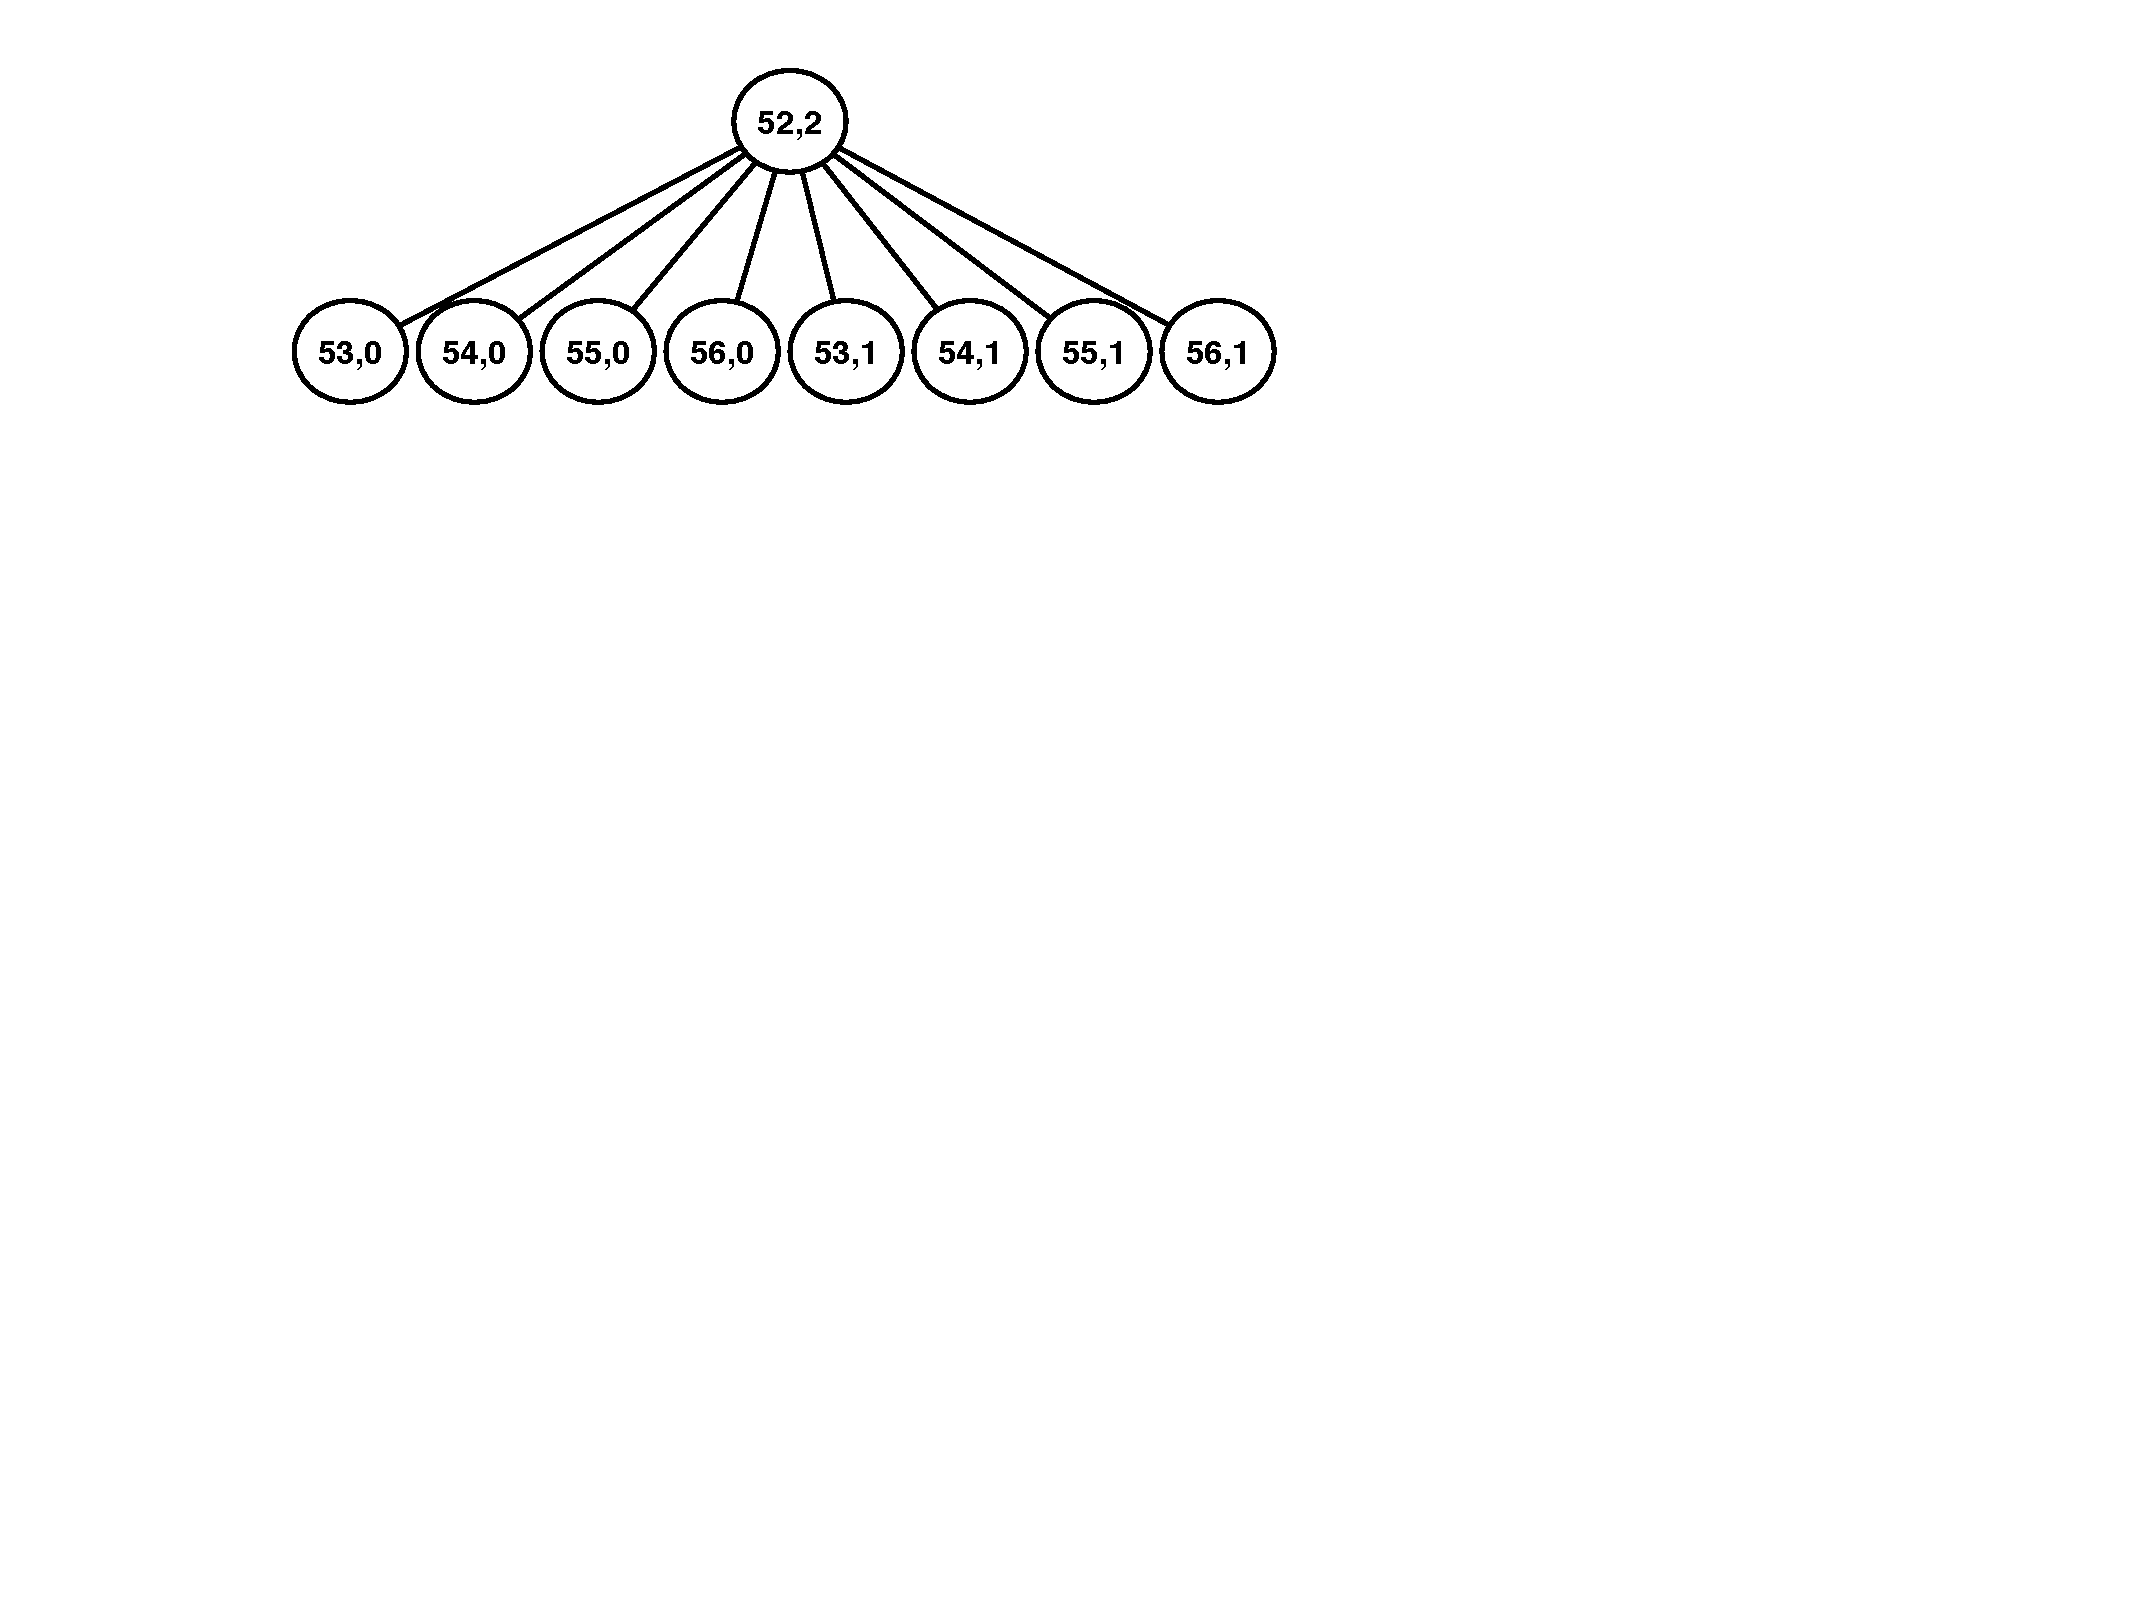
\includegraphics[width=60mm]{./Figures/bitTricks.pdf}
				\caption{An internal node with (simplified) label (52,2). The second number indicate that its $1/2$-approximation is  $2^2 = 4$. The children are given labels in  $\{53 \dots 56\}$ and an additional bit. }
				\label{fig:bitTricks}
			\end{figure}
			
			
 

%Suppose node $v \in T$  with traversal number $\dfsi(v)$ has $i$ children $c_1 \dots c_i$, and denote v's $1/2$-approx  $\lfloor v \rfloor $.
%Nodes $c_1 \dots c_{\lfloor v \rfloor }$  are given a label composed of their corresponding traversal number from $ \dfsi(v)+1 \dots \dfsi(v)+ \lfloor v \rfloor$ along with an each additional bit marked $0$.
%Each node in $c_{\lfloor v \rfloor+1} \dots c_i$ receives    numbers as given by the traversal to $c_1 \dots c_{\lfloor v \rfloor}$, with their additional bit  marked as $1$.

\subsubsection{A  $\log n + O(\log^*n)$ labeling scheme}\label{sec:log-star}
To further reduce the size of the label, the authors use a special and recursive clustering on the tree $T$. 
The nice clustering  technique (Section~\ref{tec:clustering}) is modified to suit the needs of the labeling scheme.
Recall that for every $ 1 \leq x \leq n$ and any tree $T$, there exist a (nice) cluster partition dividing $T$ to  at most $n / x$ clusters, each having $O(x)$ nodes.
\begin{definition}
A cluster $C(u,v)$ (Def.~\ref{dfn:cluster}) is a \emph{single child cluster} if 
\begin{inparaenum}[\itshape  I.\upshape)]
\item it is a leaf cluster; or
\item it  contains at most two nodes; or
\item $u \leadsto v$ contains at least 5 nodes, $v$ has no children in $C(u,v)$, and $u$ has only one, i.e., the node on the path to $v$.  
\end{inparaenum}
A nice cluster partition   (Definition~\ref{dfn:nice-cluster-partition})  is a \emph{single child cluster partition} if all its clusters are single child clusters.
\end{definition}

We complete an omitted   proof of  Lemma 7  in~\cite{Alstrup02}. 
\begin{lemma}\label{lemma:nice_decomp}
Let $T$ be a rooted tree with $n$ nodes. For every  $ 1 \leq x \leq n /7$ there exist a single child cluster partition of $T$ of at most $n/x$ clusters, each containing $O(x)$ nodes.
\end{lemma}

\begin{proof}
Let $\cs$ be a  nice cluster partition for $T$ with $\vert \cs \vert \leq n/7x$ and each cluster contains $O(x)$ nodes.
We decompose every  internal cluster $C(u,v) \in  \cs$ which is  not a single child cluster to at most  seven single child clusters as described below. 

Assume  that $u \leadsto v$ contains 5 or more nodes, and  that  $v$ has  children in  the cluster $C(u,v)$. Denote an arbitrary child of $u$ not on $u \leadsto v$ as $u'$.
 $C(u,v)$ is decomposed to  the clusters $C'(u,v)$ and $C'(u,u')$, where $C'(u,u')$ is a leaf cluster consisting of the  children of $u$ excluding the one in the path $u \leadsto v$, and $C'(u,v)$ contains the rest of the nodes.
We use a similar procedure on  a cluster $C(u,v)$ where $v$ has more than one child.
It follows that a cluster $C(u,v)$ is decomposed to  at most two leaf clusters and one internal cluster $C'(u,v)$ that contains the path $u \leadsto v$.
Hence, all three clusters are single child clusters.

If  $C(u,v)$ contains more than two nodes, and  $u \leadsto v$ contains less than five, we decompose the cluster  in the following manner (illustrated in Figure~\ref{fig:crazyeleven}).
An internal 2 node cluster $C(i,j)$ is created for every two adjacent nodes $i$ and $j$ on the path $u \leadsto v$.
In addition, a leaf cluster $C(a,b)$ is created  for every node $a$ on $u \leadsto v$  with at least one child not on the path.
Let $\mathcal{F}_d$ be the forest created by removing all edges on the path $u \leadsto v$ from the cluster $C(u,v)$.
Each cluster contains all the nodes in the tree rooted in $a$ from $\mathcal{F}_d$, and $b \neq a$, an arbitrary  node in $\mathcal{F}_d$.
To conclude, $C(u,v)$ is transformed to at most three single child internal clusters, and at most four leaf clusters.
\end{proof}

				\begin{figure} 
				\centering
				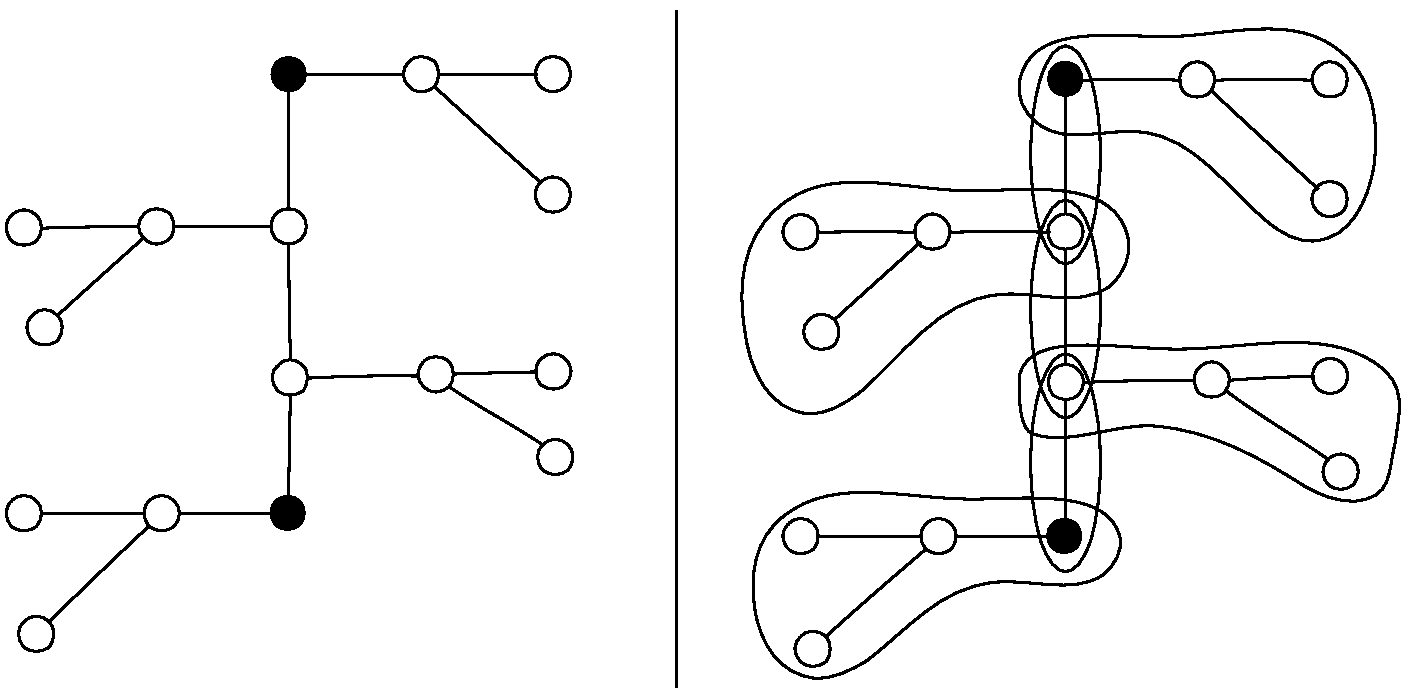
\includegraphics[width=80mm]{./Figures/7.pdf}
				\caption{Left: A nice cluster, Right: the cluster decomposed to 7 single child nice clusters. Black nodes are boundary nodes.}
				\label{fig:crazyeleven}
			\end{figure}
			
			

The cluster partitioning guaranteed in Lemma~\ref{lemma:nice_decomp} is used to  create a correlating \emph{macro tree}.
\begin{definition}\label{dfn:macro-tree}
A cluster partition $\cs$ has  a \emph{macro tree} $T_m$ defined as follows. 
The nodes $V(T_m)$ are the set of boundary nodes of  $\cs$.
The edges $E(T_m)$ are the set of pairs $(u,v)$, where $u,v$ belong to the same cluster $C(u,v)$. 
The root of $T_m$ is the root $r$ of the original tree $T$.
This is possible since $r$  is defined to be a boundary node of some cluster in $\cs$.
\end{definition}


			
			
\begin{theorem}\label{theo:adjacencytreesupper}\cite{Alstrup02}
There exist an \adjacency labeling scheme for $Trees(n)$ whose worst-case label size is at most $\log n + O(\log^* n)$.
\end{theorem}

\begin{notproof}[ sketch]
We begin by  labeling the macro tree $T_m$ (Def.~\ref{dfn:macro-tree}) of a single child cluster partition of $T$, using the  leaf favouring encoder $e_\beta$ (defined in  Lemma~\ref{lem:4loglogn}).
Every edge $(u,v) \in E(T_m)$ represents a \emph{micro tree}, a cluster  of at most $cx$ nodes, for some $c$, not including its boundary nodes.
In addition, $T_m$ has at most $n/x+1$ nodes.
We can use  $e_\beta$ to encode the leaves of $T_m$ using $\log(n/x)+O(1)$ bits, and the inner node of $T_m$ using $\log(n/x)+4\log\log(n/x)$. 
By choosing $x = \log^5 n$ both label sizes are bounded by $\log n + O(1)$.  
For the remainder of the proof, an edge $(u,v) \in E(T_m)$ where $\dfsi(u)<\dfsi(v)$ is labeled in $v$'s label,  $\la(v)$.

Consider the  nodes  in the internal cluster $C(a,b) \setminus \{a,b\}$.
These nodes maintain adjacency relation only between themselves and possibly the two boundary nodes $a$ and $b$.
By storing only a unique identifier of the edge they belong to in the macro tree, we can safely reject a query of two nodes from different clusters.
 Such a unique label is already given to every micro-tree labeled $\la(b)$  by $\dfsi(b)$, which is just the first $\log(n/x)$ bits of the label given by $e_\beta$. For illustration, see Figure~\ref{fig:Clustering}.
We stress that  the non-boundary nodes of the internal clusters are exempt from maintaining the additional $4\log\log(n/x)$ bits required by $d_\beta$ to determine \adjacency in $T_m$. 
We now mark the  boundary nodes, and their immediate (single) neighbours from each side by a finite number of types (such as root of an internal cluster, a child of a root of a cluster etc.).

				\begin{figure} 
				\centering
				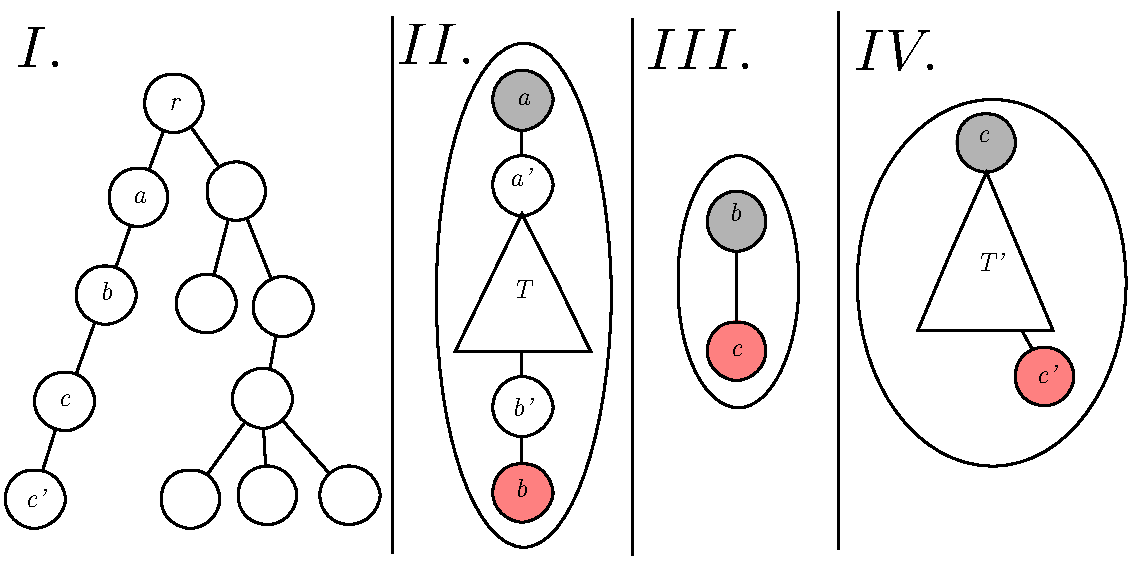
\includegraphics[width=90mm]{./Figures/MacroTreeNew.pdf}
				\caption{From left to right: \begin{inparaenum}[\itshape  I.\upshape)]
\item  A  macro tree $T_m$ with boundary nodes $a,b,c,c'$;
\item the internal cluster $C(a,b)$;
\item the internal cluster $C(b,c)$; and
\item the leaf cluster $C(c,c')$.  
\end{inparaenum} According to the labeling scheme the nodes in $T$ rooted by $a'$ store only the unique identifier of node $b$ in $T_m$, rather than the entire $\la(b)$ assigned to the node in $T_m$.  The last node in the $\dfsi$ traversal of $T$ is $b'$. }
				\label{fig:Clustering}
			\end{figure}
			
A full label for the tree is achieved by concatenating those labels with the \adjacency labels of  the micro trees, using the original   $\log x + 3\log \log x$  bits labeling scheme for trees of size $x$. This time  the boundary nodes  are the one exempt from  storing this information. The decoder can detect if  two nodes are in the same micro tree using the first part, and  check for \adjacency if the  two nodes  are in the same micro part, using the  second part of the labels. 

To summarize, there are now four types of nodes. Nodes in  leaf clusters, boundary nodes of the internal clusters, immediate neighbors of the boundary nodes, and nodes in micro trees of internal clusters.
All four now enjoy a labeling scheme of at most $\log n + 3 \log \log \log^5 n+ O(1)$.  

At this point the authors utilise the structure of the new micro trees and label those by applying the labeling scheme recursively.
The encoder  assigns $\la(u)$ to $u \in T$ as a concatenation of at most $i$ decreasing size macro trees that contain $u$.
The last element concatenated to $\la(u)$ marks that $u$ is  either be a boundary node in some level prior to $i$, or a full label of $u$ in the last micro tree.
Denote $f(n) = log^5(n)$ and $f^i(n)$ operating $f$ $i-1$ times recursively on $n$.
$e_\beta$ is applied $i-1$ times, and nodes in the (final) micro trees are labeled by the second encoder $e_\alpha$.
The  description of  the labeling scheme  yields  labels of size at most:
\begin{dmath}
	 \sum_{j=1}^{i} \left( \log{(f^{j-1}(n)/f^{j}(n))} + O(1) \right) + 3\log \log{(f^{i-1}(n)/f^{i}(n)}) +O(1)  = \log{n} + \log{f^i(n)} +  i \cdot O(1) + 3\log \log{(f^{i-1}(n)/f^{i}(n))}. 
\end{dmath}
Assigning $i= \log^* n$ we have that the maximum label size is $\log n + O(\log^* n)$ as guaranteed.
\end{notproof}


\subsection{Traversal and jumping}\label{traversaljumping} 			
			Caterpillars were shown to have a labeling scheme of $\log n+{O}(1)$ by \citeN{Gavoille06},  using a technique called ``traversal and jumping". In the remainder of this section we occasionally refer to the labels as the integers they represent.
			
A caterpillar tree $T$ rooted in $x_1$ consists of the  path  of \emph{internal nodes} $P = x_1 \dots x_{p}$ where each $x_i \in P$ has $l(i)$ \emph{leaf children} $L(i) = y_1^i \dots y_{l(i)}^i$.
The only two cases where two nodes are adjacent in a caterpillar is either when one is a leaf child of the other or if they are  adjacent internal nodes. 
We also note that  there exist a straightforward  non-unique \adjacency labeling scheme for this family.

Recall that  a $\dfsi$  traversal (Section~\ref{sec:efficient-encoding}) of a   caterpillar $T$  rooted in    $x_1$ visits nodes in $L(i)$ before  $x_{i+1}$ for all $1 \leq i \leq p $. As with the labeling scheme in Section~\ref{sec-adj-lb}, the leaves do not contain additional information other than a unique identifier. For every $1 \leq i \leq p $ and $1 \leq   j \leq l(i)$, we set $\la(y_j^i) = \la(x_i)+ j$.  In other words, the leaf children of $x_i$ are given labels  consecutively after $x_i$'s label, and a single bit is  prefixed to each label to determine the node's type.  

 We can construct a  $2 \log n$  \adjacency labeling scheme by assigning $\dfsi(v)$ to every node $v$, and concatenate    $l(i)$ to  every internal node.
 An internal node $u$ and a  leaf child $v$ are adjacent if and only if  $\dfsi(u) \leq \dfsi(v) \leq \dfsi(u)+l(i)$, and two internal   nodes $u$, and $v$ where $\dfsi(v)>\dfsi(u)$ are adjacent if and only if  $\dfsi(u)+l(u)+1= \Id(v)$.
 
Rather than storing  $l(i)$ in $x_i$, we  maintain a 2-approximation (Section~\ref{tec:approx}) of both $l_i$ and $l_{i+1}$ denoted 
$\ceil{l_i}_2$ and $\ceil{l_{i+1}}_2$, respectively in $x_i$. For $1 \leq i \leq p$ we compute  $$t_i := max\{ 2 \log{t_{i+1}}, \log(\ceil{l_i}_2 )\}+O(1),$$ where $t_{p} =  \log(\ceil{l_p}_2)$. An  internal node $x_i \in P$ is assigned a range of size $2^{t_i}$ in which the label of $x_i$ and the labels of $L(i)$ will reside.  
In order to store both $t_i$ and $t_{i+1}$ in the label of $x_i$, we first construct the suffix code (Section~\ref{tec:suffix}) $C(x_i)$, which is defined as:
$$C(x_i)= code_1(t_{i+1}) \circ code_0(t_i - \vert code_1(t_{i+1}) \vert ).$$
We  then choose the  label of $x_{i+1}$ to be   the  number in the range  
$\{\la(x_i)+2^{t_i} \dots \la(x_i)+2^{t_i} + 2^{t_{i+1}}\}$ that  contains $C(x_i)$ as a suffix.
 We find this particular number using Lemma~\ref{lemma:numberinside}. Due to the selection of $t_i$, it is guaranteed that there are at least $l(i)$ consecutive numbers in the range after that number.
To prove that the size of the label  is at most $\log n + O(1)$ the authors prove that for some constant $c'$:
 $\sum_{i=1}^p 2^{t_i} \leq  c' \cdot \sum_{i=1}^p l(i)$. 
 %For completeness the proof is given in Appendix~\ref{AppendixC}.
  Since $\sum_{i=1}^p l(i) < n$, it follows that the maximum label size used by any internal node is $\log n +O(1)$.  
 The largest label is assigned to the last leaf $\la(y_{l(p)}^p)$, and since the leaves are assigned numbers consecutively after their parents, the number of labels is at most doubled, requiring only one additional bit. For an illustration of the technique see Figure~\ref{fig:caterpillar}.


				\begin{figure} 
				\centering
				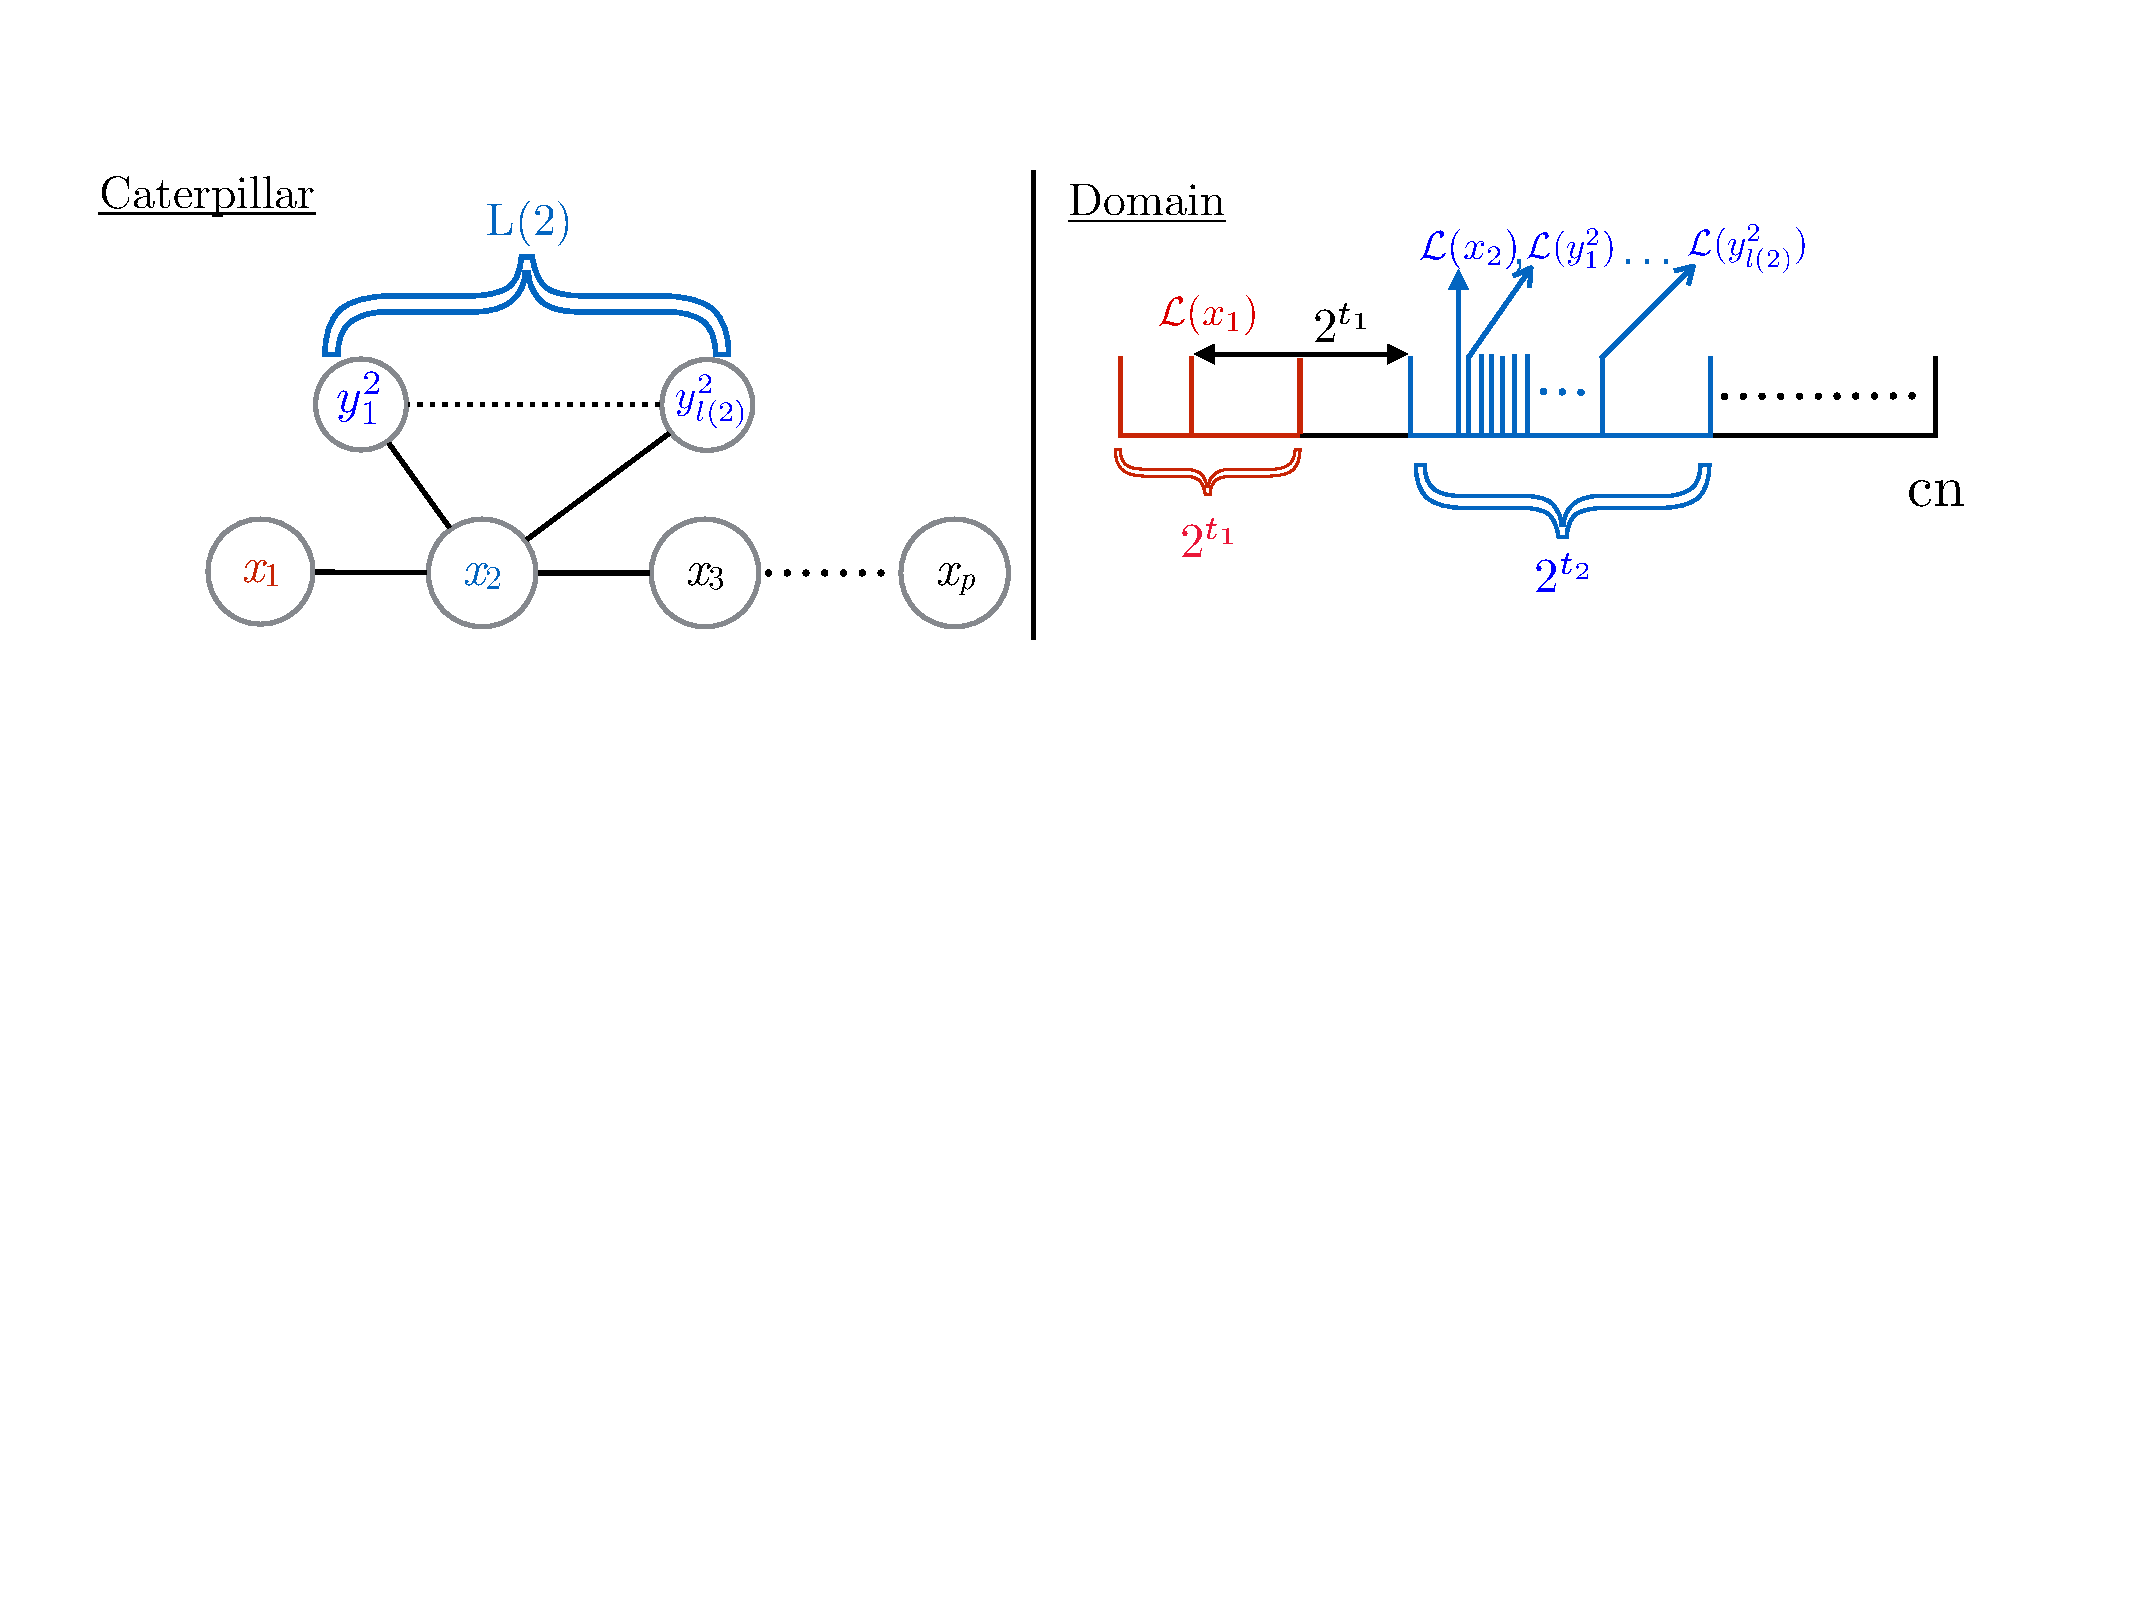
\includegraphics[width=120mm]{./Figures/Caterpillars.pdf}
				\caption{Label assignment of the inner nodes and leaves of the caterpillar depicted on the left using traversal and jumping. 
				The label  $\la(x_1)$ is chosen from $\{1 \dots 2^{t_1} \}$,  $\la(x_2)$ from $\{\la(x_1)+2^{t_1} \dots\la(x_1)+2^{t_1}+2^{t_2} \}$ and the  leaves $y_1^2 \dots y^2_{l(2)} \in  L_2$ are labeled s.t.  $\la(y_1^2) = \la(x_2)+1 \dots  \la(y^2_{l(2)}) = \la(x_2)+ l_2$.}
				\label{fig:caterpillar}
			\end{figure}


\paragraph{Optimal bounded degree}		
		Recently, \citeN{adjiashvili2014labeling} proved the existence of a labeling scheme for  $Trees(n, \Delta)$ with label size of  $\log n+O(\log \Delta)$.
		The labeling scheme is based  on an embedding technique of Bhatt, Chung, Leighton and Rosenberg~\shortcite{BCLR}.
		Bhatt et al.  showed the existence of an induced universal graph with   $O( \Delta \cdot  n)$  nodes that contains the family $Trees(\Delta,n)$. Although the construction was explicit, it is unknown how to produce efficient  decoder to match the possible encoding suggested by the construction.
		
		 \citeN{adjiashvili2014labeling} noticed that the simple construction in \cite{BCLR} (Lemma~3)  can produce a $\log n +O(\Delta)$ labeling schemes for the family, where the label is a concatenation of a node and edge identifiers.
		 More precisely, the label $\la(u)$  of node $u$ with parent $w$, has two parts: $u$'s unique number and the  local number of the edge $(u,w)$ in the universal graph.
		 The major problem is to determine at which point in the binary  string the first part  stops and the second part starts. To that end the authors used the label size as an additional input for the decoder.

\subsection{One-sided error \adjacency labeling scheme}\label{sec-adj-onesided}
		Consider the function \nonadjacency  for any graph $G= (V,E)$ that returns true if and only if  nodes $u,v \in V$   are \emph{not} adjacent in $G$.
		Suppose we  demand  our query to be precise only  when the nodes are in fact adjacent, and allow two non adjacent nodes to be declared adjacent.
		It is of course helpful to be able to predict and control how often such a ``false positive'' would occur.
		\cite{fraigniaud2009} demonstrate the usefulness  of one-sided error labeling scheme (Definition~\ref{dfn:one-sided}) for \adjacency in the following.	
			\begin{theorem}
			For any $1 \leq k $ there exist a one-sided error \nonadjacency labeling scheme  $\tuple{e,d}$  for $Trees(n)$ with guarantee $p = 1- \frac{1}{2^k}$ of size $2(k+1)$.
			Furthermore, $e$ is computed in $O(n)$, and $d$ is computed in $O(1)$
			\end{theorem}
			\begin{proof}
			For each node $v \in V$ in the tree $T=(V,E)$, $e$ assigns  $\la(v) = \tuple{\la_1(v),\la_2(v)}$  as follows.
			 The root $r$  is assigned $\tuple{\la_1( r ), \la_2( r )}$, where $\la_1( r )$, $\la_2( r )$ are chosen uniformly at random in  $ \{0 \dots 2^{k+1}-1 \}$. 
			A node $u$ with parent $v$ in the tree is assigned $\la_1(u) = \la_2( v )$ and $\la_2( u )$ chosen uniformly at random in  $ \{0 \dots 2^{k+1}-1 \}$. 
			 $e$ is clearly computed in $O(n)$ with $n+1$ calls to a random function, and may assign non-unique labels.
			 
			 The decoder $d$ will decode $ \tuple{\la_1( u ) , \la_2( u )},\tuple{\la_1( v ) , \la_2( v )}$  by evaluating  the predicate  $(\la_1( v ) =  \la_2(u))  \vee  (\la_1( u) =  \la_2(v)) $.	
			  If $u,v \in V$  are  adjacent, the predicate is trivially  satisfied.
			 If $u,v \in V$  are  non adjacent, $prob(\la_1( v ) =  \la_2(u)) = prob(\la_2( v) =  \la_1(u)) = \frac{1}{2^k+1}$.
			 Therefore, the predicate is satisfied with probability
			  $\frac{1}{2^{k+1}} + (1 - \frac{1}{2^{k+1}})\cdot \frac{1}{2^{k+1}} < \frac{2}{2^{k+1}} = \frac{1}{2^k}  $
			  , and thus $p = 1-\frac{1}{2^k}$.	
			  \end{proof}
			Notice that one bit is sufficient to avoid  false determination of two  adjacent nodes as  non adjacent.
			The latter theorem shows that for ``false positive''  guarantee of   $99.99\%$, as few as 30 bits are sufficient.
			Choosing  $k= \log n+O(1)$  ensures  a guarantee   $p = 1-\frac{1}{2^{O(1)} \sqrt{n}}$. In contrast, \citeN{fraigniaud2009} prove that any  one-sided error  \adjacency labeling scheme for $Trees(n)$  with guarantee $p$ requires labels of  size at least  $\log n + \log p - O(1)$. 